
%!TeX spellcheck = en-US
%\chapter{Word Embedding and Distributional Features of the web-pages and texts}
\chapter{Open-set WGI with Distributional Features}

\label{chap:word_embeddings}


%----------------------------------------------------------------------------------------

% Define some commands to keep the formatting separated from the content
\newcommand{\keyword}[1]{\textbf{#1}}
\newcommand{\tabhead}[1]{\textbf{#1}}
\newcommand{\code}[1]{\texttt{#1}}
\newcommand{\file}[1]{\texttt{\bfseries#1}}
\newcommand{\option}[1]{\texttt{\itshape#1}}

%----------------------------------------------------------------------------------------

\section{Introduction}\label{chap:word_embeddings:sec:intro}
 
 

\section{N-grams, Word Embeddings and Distributional Features} \label{chap:word_embeddings:sec:ngrans_vs_doc2vec}


The Bag of Terms (BOT) n-grams, a.k.a the Bag of Words (BOW), is the most common text modeling in NLP and other text related research domains. The assumption as in other features from other domain, say image processing, is the \textit{Independent and Identical Distribution (i.i.d)} of the terms, then it is easy to express context of a text into a \textit{fixed vector} sample which is the main requirement of most ML algorithms to work. Moreover, is computationally very easy and in the past the creation of such a fast document representing in respect of time consumption was critical due to the lack of the today's resources.

The BOT is still a top performance document representation however it comes to a great cost because it is loosing the order of the words and cannot capture their semantics. Therefore, it is impossible to capture similarities in word level such as "power" and "strength", in sentence level such as "Beats me!" and "I don't know", and in writing style such as "My greetings to..." and "Say hello to... for me". 

\textit{Word Embeddings} and \textit{Distributional Feature (DF)}s is the state-of-the-art in language modeling as a result in the advances of the \textit{Statistical Language Modeling} and particularly the \textit{Neural Probabilistic Language} modeling. Ultimately, the \textit{Paragraph Vector Continues Bag of Words (PV-BOW)} DF modeling can be used for complicated classification tasks such as WGI, where the BOT together with its complicated heuristics for additional feature extraction can only perform as good when the task is more tight the corpus. Although, as it will be explained later the DF models and word embeddings is a computationally expensive process is might be comparable to a sequential set of heuristics for extracting a variety of features in the effort of capturing the information missing from the BOT in the first place.  

In this section it is described the PV-BOW modeling in detail, which have been used in combination with the NNDR (the open-set Nearest Neighbours) on the WGI task with promising results. First, it is described the \textit{Neural Language Modeling (NLE)} concept and on the top of it the \textit{Continues Bag of Words  (CBOW)} and  \textit{Skip-Gram (SG)} modeling, which they are special modified \textit{Feedforward} and \textit{Recurrent Neural Network models respectively}.

The goal of \textit{Statistical Language Modeling (SLM) } is to learn \textit{joint probability distribution function} of word sequences, i.e. word n-grams. The main difference to the BOW and particularly to the word n-grams TF (or TF-IDF) model, is the \textit{semantic proximity} of the word's neighbouring in the sentences. Implicitly the WNG-TF models is also capturing some of this information and definitely not explicitly. Additionally, the SLM can always return an estimate value for n-grams never seen before, while for the WNG-TF this is impossible  \parencite{bengio2003neural}

The SLM model is defined as the \textit{joint conditional probability distribution} of the next word given the probabilities of previous ones as shown in equation \ref{chap:word_embeddings:eq:slm}

\begin{equation} \label{chap:word_embeddings:eq:slm}
	P(w = i) = \prod_{i=1}^{|V|} P(w_{i}|w_{i-k}, ... , w_{i+k})
\end{equation}
\noindent
where $w_{i}$ is the i-th word, and $k$ is for the number of words before or/and and after, writing sub-sequence $w_{i} = (w_{i-k}, w_{i-1}, ... ,w_{i+1}, w_{i+k})$. Note that this model returns a singleton value for a word on the condition of previews or/and next word. This model also can be expanded to have few more words in the conditional probability, usually from 2 up to 4. 

With this model it can be captured the semantic proximity but it will return zero in the case a sequence have never been met before in the samples. A solution to this problem is the interpolation or smoothness factor that can be applied such as in the \textit{back-off tri-gram model} (Katz, 1980 see in bengio2003neural). 

The model of equation \ref{chap:word_embeddings:eq:slm} can capture the joint probability of word-sequences in terms of feature vectors, however, it cannot capture the correlation of the words in terms of semantics. Models like LSI or LDA are methodologies also been tested in IR and NLP for capturing the semantics in the context of the n-gram based SLM. 

The goal of the DF models is to learn simultaneously the \textit{word feature vectors}, a.k.a \textit{Word Embeddings}, and the probability function or word sequences, a.k.a \textit{Distributional Features}. The word embeddings is a \textit{continuous vector space} where the words are positioned in \textit{Vocabulary} context, where the similarity of words can be learned. The word sequences are capturing the proximity of words in the paragraph (or sentence) context.

The DF models then are able to learning the \textit{Continuous Distribution of Words in Sequences} and not only their role in sentences (such as in eq.  \ref{chap:word_embeddings:eq:slm} model) or only their similarity (such as the LSI models). The DF modeling is a NLM procedure where Neural Networks are used for approximating the\textit{ joint probability distribution function of the continuous distributed feature-sequences}, where the probability features are associated to the words of the Vocabulary.

In practice the distributed features is the mapping of the Vocabulary words $V = \{w_{i}, i \in [1, |V|] \}$ to a real vector $\vec{t}(i) \in \mathbb{R}^{m}$. Then the semantic distance can be approximated by a NNet algorithm given the distribution of the words. The words are initially are having a vector 1-of-V representation, a.k.a. \textit{One-hot representation}. Then the probability of the a word $w_{i}$ in equation \ref{chap:word_embeddings:eq:slm} can be replaced by the real continues vector $t{i}$ and the conditional probability $P(.|.)$ to be approximated my a NNet function $\hat{p}(.)$. The $\hat{}$ (hat) is for symbolizing a special condition where the probability is approximated given a sequence with a specific order, say preceding words or succeeding words or both. 

Now the DF neural model can be calculated with several architectures where the $\vec{t}$ and the $\hat{p}$ continues distribution can feed separate layers of joint layers, and also the learning strategy can have variant implementations such as Continues Bag-of-Words, Skip-grams etc. The strategy of learning and the NNet architecture are very close related and the results are \textit{continues probability functions with substantially different meaning}, where they can either encode word similarities, word semantics or even paragraph and documents encoding and similarities. 

To begin with, the most general architecture is to use the \textit{Feedforward Neural Network} with a projection layer, a hidden layer and an output layer as shown in figure \ref{chap:word_embeddingss:fig:CBOW_diagram}. This NNet has an input layer where every word in the vocabulary is assigned to an One-hot vector $\hat{t}_{i}$ and all the sequence of the \textit{word vectors} are concatenated and forming the input vector $\hat{w}_{i}$ . The $\hat{w}$ is the input the projection layer $\vec{t} = \hat{w}W_{in}$ as show in the figure. The $W_{in}$ is the weight matrix of the projection layer with same regularization parameters $\theta$.

\begin{figure}[t]
	\begin{center}
    	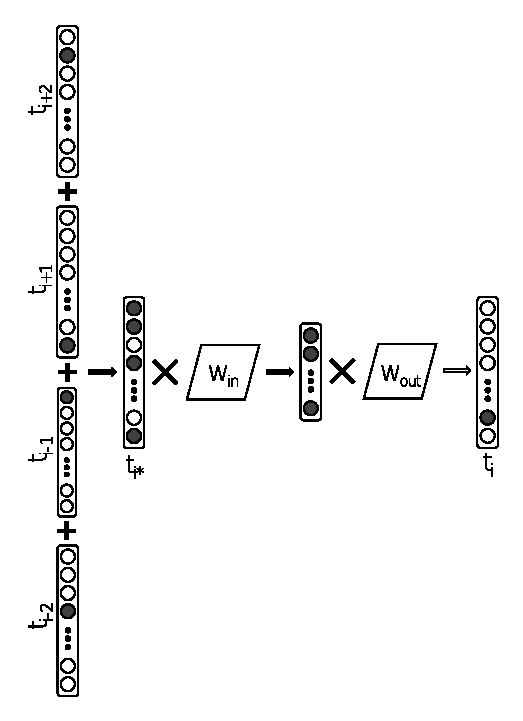
\includegraphics[scale=0.99]{Figures/CBOW_diagram.eps}
		\caption{Diagram for C-BOW and General NLM architecture. Depending whether the $t_{i*}$ is part of the projection and the hidden layer or the layers are different. In practice the weighting matrices are either shared or diff rent between the word projection and the hidden layer or it is the same matrix, which is equivalent to the words been projected to the same position as their vectors are averaged and not concatenated.}
		\label{chap:word_embeddingss:fig:CBOW_diagram}
	\end{center}
\end{figure}

Now the $\vec{t}$ is the input to a hidden layer $\vec{h}=\vec{t}H$, which is usually the \textit{hyperbolic tangent hidden layer}, where $H$ is the weights of the hidden layer. Then, the output $\hat{p}=\vec{h}W_{out}$ is the last layer of the NNet.

The generic architecture of the final output of the NLM described above is the equation \ref{chap:word_embeddingss:nlm_generic}. Note that the output vector $\vec{y}$ has size $|V|$ due to the input $\hat{w}$ and is the inference model of a \textit{continues distribution} of both the proximity of the words in the sentences (captured by the hidden layer) and the distribution over the vocabulary, which is the continues similarity of the words in this vocabulary. The output layer then is as described in equation \ref{chap:word_embeddings:eq:NLM}

\begin{equation} \label{chap:word_embeddings:eq:NLM}
	\vec{y} = \vec{t} + W_{out}(\vec{t}H + b_{h}) + b_{o}
\end{equation}

\noindent
where $b_{o}$ and $b_{h}$ are the output and hidden layers biases. Usually the Hidden layer typically has a size of 500 to 1000 neurons while the projection layer might be 500 to 2000. Due to the multiple layers and the feeding of both the projection and the hidden to the output layer there is great complexity and the process is very computationally demanding. 

A more efficient method is suggested in \parencite{mikolov2013efficient} where the non-linear hidden layer is removed and the projection layer is shared to all words, geometrically this is equivalent to the projection of the words to the same position. Then the algorithm is reformed and the $\hat{w}$ vectors are replaced by the $t^{*}$ which is the sum of the \textit{one-hot word vectors} \parencite{mitra2018introduction}. 

Now the equation \ref{chap:word_embeddings:eq:NLM} is becoming \ref{chap:word_embeddings:eq:CBOW}. Due to the new form of the NNet where the tangent hidden layer is absent, there is no constraint in the presenting sequence of the words order. Moreover, the succeeding words also can also be taken in to account in a given \textit{window} say for $k_{w}$ number of words around the specific one. 

\begin{equation} \label{chap:word_embeddings:eq:CBOW}
	\vec{y} = W_{out}(t^{*}W_{in}) + b_{o}
\end{equation}
The suggested algorithm is called \textit{Continues Bag-of-Words (CBOW)} because the words of the surrounding sequences is not important but it is still are taken into account for predicting the next word. Moreover the $\vec{y}$ has a size equivalent to the size of the Vocabulary $V$. 

In respect of training the CBOW model, a \textit{multiclass classifier} is set by a \textit{Softmax function} is described in equation \ref{} where the $y$ is the output of the equation \ref{chap:word_embeddings:eq:CBOW}. Note now the $\hat{p}$ continues probability is replaced by the $p$ district probability and because now the order in the words sequences are not important. Additionally, the $\vec{t}$ are replaced by the $t$ because it denotes that the words can be any term; character, words, word n-grams, character n-grams. 

\begin{equation} \label{chap:word_embeddings:eq:CBOW_softmax}
	p(t_{i}|t_{i-k},...,t_{i+k}) = \frac{e^{y_{t_{i}}}}{\sum^{|V|}_{i}{e^{y_i}}}
\end{equation}

The objective of the training of the NLM CBOW model is to maximize the conditional log probability in equation \ref{chap:word_embeddings:eq:CBOW_log_likelihood}. 

\begin{equation} \label{chap:word_embeddings:eq:CBOW_log_likelihood}
	 \mathcal{L}_{CBOW} = \frac{1}{|S|} \sum_{i=1}^{|S|}{\log{p(t_{i}|t_{i-k}, ... ,t_{i+k};\theta)}}
\end{equation}


\noindent
where $S$ is the \textit{set $k$-size of sampling windows} and  $\theta=\{b_{o},W_{in},W_{out}\}$ are the parameters and weights should be optimized in order the CBOW model to converge. \textit{Stochastic Gradient Decent} and \textit{Backpropagation} is used for training the NNet.

An other training strategy is the \textit{Skip-Gram} modeling, where the objective is to maximizes the log-likelihood of the equation \ref{chap:word_embeddings:eq:skipgram_log_likelihood}.

\begin{equation} \label{chap:word_embeddings:eq:skipgram_log_likelihood}
	 \mathcal{L}_{SkipGram} = \frac{1}{|S|} \sum_{i=1}^{|S|}{ \sum_{-k \leq j \leq +k}{ \log {p(t_{i+j}|t_{i};\theta)}  } }
\end{equation}
\noindent
where $S$ is the prediction windows over the training text and $k$ is the number of the words to be predicted surrounding the input word $\theta$ set of parameters to be optimized. The Softmax function of equation \ref{chap:word_embeddings:eq:skipgram_softmax} is applied at the output layer.

\begin{equation} \label{chap:word_embeddings:eq:skipgram_softmax}
	p(t_{i+k}|t_{i}) = \frac{ e^{(W_{out}  \times  t_{i+j})^{T} (W_{in} \times  t_{i})}}{\sum^{|V|}_{i}{ e^{(W_{out}  \times  t_{k})^{T} (W_{in} \times  t_{i})}}} 
\end{equation}
As shown in figure \ref{chap:word_embeddingss:fig:skipgram_diagram} the input and the output are one-hot vectors.

\begin{figure}[t]
	\begin{center} 
    	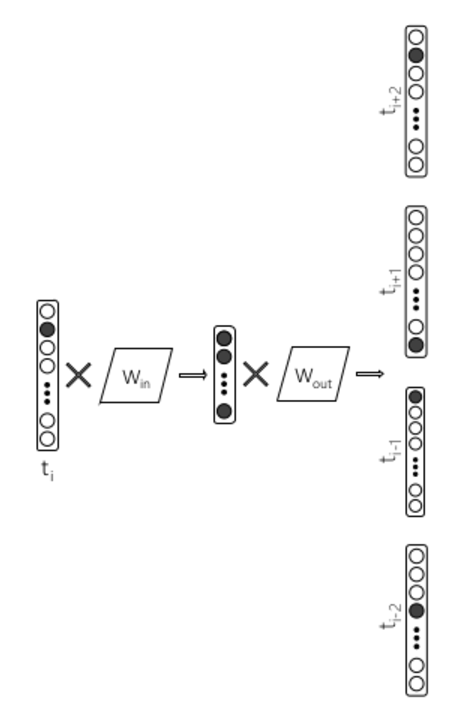
\includegraphics[scale=0.99]{Figures/skip_gram.eps}
		\caption{Diagram for Skip-Gram.}
		\label{chap:word_embeddingss:fig:skipgram_diagram}
	\end{center}
\end{figure}


Note that the two different weight matrices $W_{in}$ and $W_{out}$ (similarly to the CBOW) constitutes the $\theta$ set of parameters to be optimized of the models. $W_{in}$ gives the "in" embeddings corresponding to the input terms and $W_{out}$ corresponds to the output embeddings for the output terms. $W_{in}$, a.k.a. \textit{Word Embedding}, are used for several IR and NLP classification and regression tasks. The $W_{out}$ are usually discarded. 

A very important difference between the CBPW and Skip-Grams is the NNet architecture usually their implementation is based. Particularly, there are some internal detail occurring because of the objective ot the task. \parencite{boden2002guide}

Finally, all the above neural models, either CBOW or Skip-Grams, since they are approximating the continues distribution probability function of words over the the Vocabulary $V$ they have the constraint described in equation \ref{chap:words_embedding:eq:nnet_constraint}

\begin{equation} \label{chap:word_embeddings:eq:nnet_condtraint}
	\sum_{i=1}^{|V|}{p(t_{i}|t_{i-k}, ... ,t_{i+k})} = 1
\end{equation}

To summarize, the NLM models such as the CBOW are very effective \textit{Language Modeling} and it has the agility to measure simultaneously several properties form the context. That is, the distribution of the terms in the paragraphs of the texts and in the vocabulary and they are also called \textit{Distributional Features}. The features are set in a continues vector space and the model can return a prediction value $y$ (see equation \ref{chap:word_embeddings:eq:CBOW}) for set of terms given as an input at the test phase of the model and they can be treated as response signals of a text. Particularly a sequence of words.

The texts also now are considered as signal and the sequence of words now has a temporal property where the proximity and the order are providing important information. In respect of the term frequencies are still considered due to the temporal properties, where now the words with the higher TF are weighting or amplifying the sequential signal input to the network.

Finally, the training of the CBOW and the Skip-gram NLM is very expensive and although they have lower complexity than the more generic Feedforward Neural Networks with the tangent hidden layer explained above. However, there are several engineering solution that are accelerating the training even more such as the \textit{Huffman Binary Tree encoding or the Words} and \textit{Hierarchical soft-max}. The later is a solution where it is enabling us to use multi-processing and the $\theta$ parameters to be updated concurrently. The parallel asynchronous updating of the parameter matrices is not conforming to the mathematical constraints however in practice the negative effect is minor. 

The\textit{ Huffman Binary Tree} is a a methods for compressing the encoding of the terms where the one with the higher frequency to be accessed faster. In addition to this, \textit{negative sampling}, {sub-sampling}, or \textit{ramdom sampling} is also used where in the range of $k$ window for surrounding words only a few are selected during training with minor effect in  performance and significant acceleration in training. 

There are several detailed studies for \textit{Neural Language Modeling (NLM)}, Distributional Features and Word Embedding in \parencite{mitra2018introduction,mikolov2013efficient,mikolov2013distributed}. In the next paragraphs is explained thea \textit{Document to Vector (Doc2Vec)} Neural Model, where it is the extension of the above models CBOW and Skip-grams. Particularly, the PV-BOW is explained which has been used in this study on WGI, where a model of  the \textit{Continues Distribution of  Paragraphs} over the corpus context. Then, the web-pages are encoded in this continues distribution and their similarity is measured for the open-set WGI.
 
 
\section{Paragraph-Vector Bag-of-Words and Document Vectors Projection}
 
In this study, the Paragraph Vector Bag-of-Words (PV-BOW) model is used for the WGI task in the open-set framework evaluation. The PV-BOW is a DF modeling of the documents as an extension of the Skip-Grams modeling. The PV-BOW extends the idea of the \textit{Continues Distribution of the Words} over the Vocabulary and the Context defined by a Corpus of documents. A \textit{Continues Distribution of the Paragraphs (CDP} is defined where this method considers the concatenation of the paragraph vector with the word vectors to predict the next word in a text window. 
 
The CDP can be derived with two methods, one is based on CBOW and the other on Skip-Grams, which is used in this study. The CBOW extension is called Distributed Memory Paragraph Vector (PV-DM) because the Paragraph Vector is given as an input together with the word vectors, and it is considered as memory of the words distribution.
 
Another way is to ignore the context words in the input, and make a model for predicting words randomly sampled from the paragraph in the output. That is the Skip-gram model but instead of a words the whole paragraph vector is given as an input as shown in figure \ref{chap:word_embeddingss:fig:PVBOW_diagram}. In practice, at each iteration of stochastic gradient descent, text window of $k$ size is sampled. Then a random word sampled from the text window and form a classification task given the Paragraph Vector and  this is the PV-DBOW. This model requires to store less data, because only the softmax weights are stored as opposed to both softmax weights and word vectors in the PV-DM. 



\begin{figure}[t]
	\begin{center} 
      	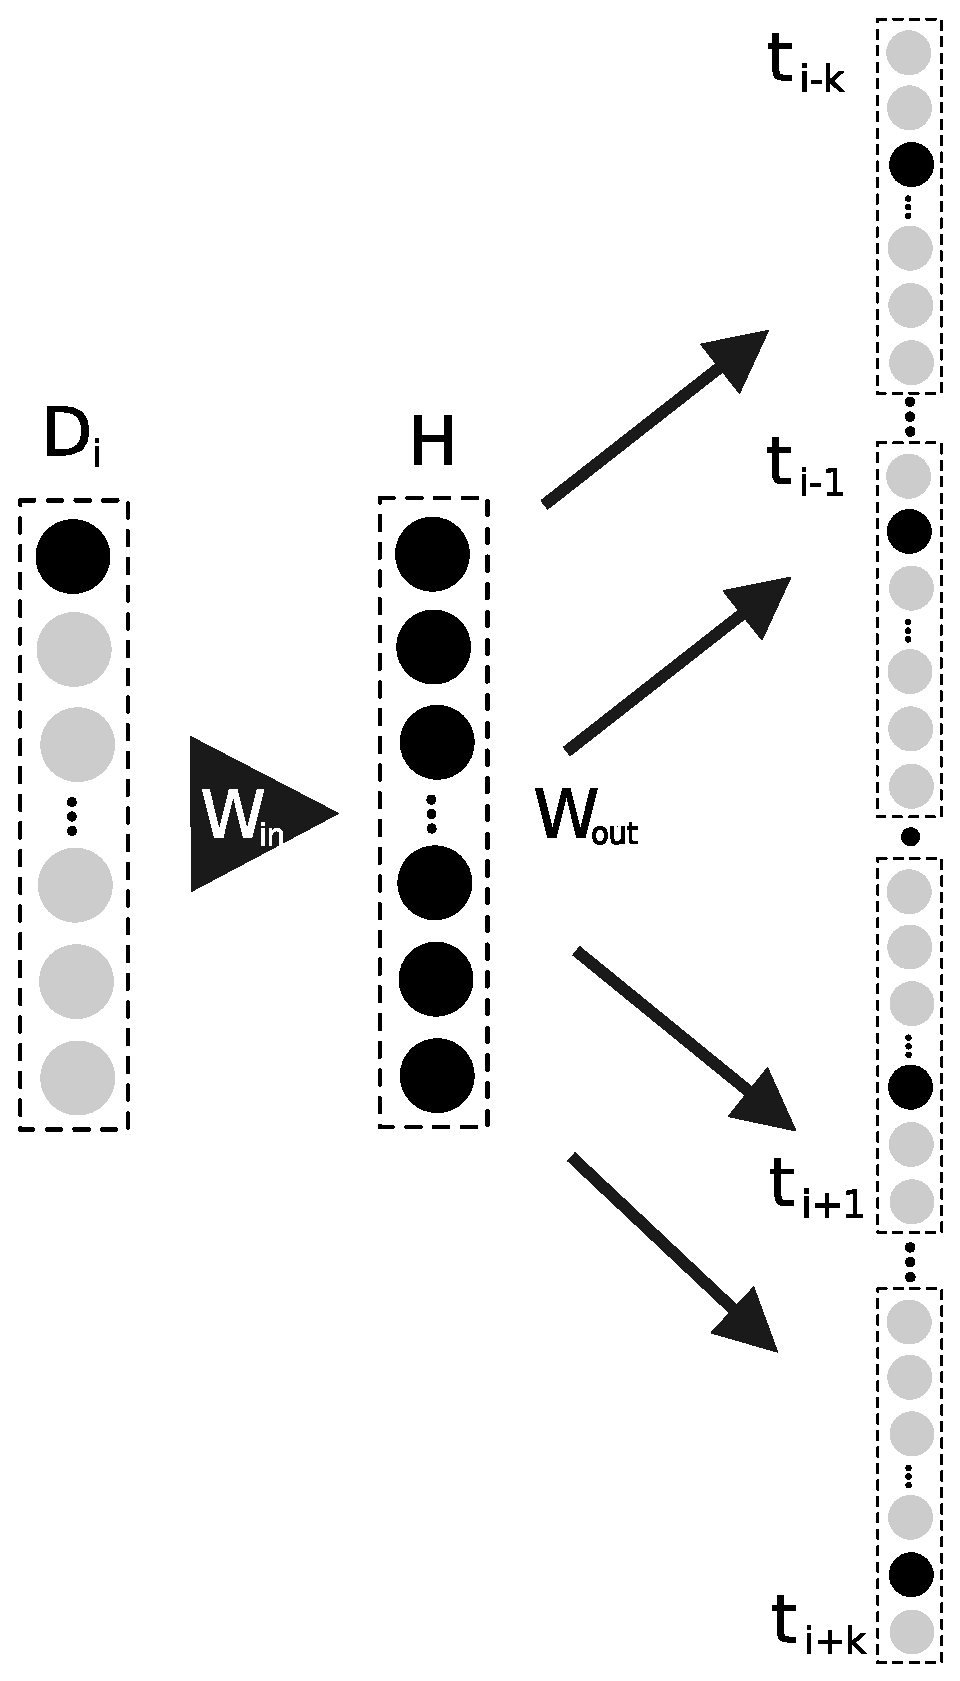
\includegraphics[scale=0.50]{Figures/pvbow.eps}
    		\caption{Diagram for PV-BOW}
		\label{chap:word_embeddingss:fig:PVBOW_diagram}
	\end{center}
\end{figure}

It should be noted that the Paragraph Vectors can be a text paragraph, a sentence, or the whole document. In this study, the whole web-pages is considered as shown in the first vector at the left in figure \ref{chap:word_embeddingss:fig:PVBOW_diagram}. There are several implementation for the PV-BOW modeling and a late evolution proposal for making the model more appreciate for IR problems. Including, \textit{Document frequency based Negative Sampling} and \textit{Document Length Regularization} \parencite{le2014distributed,posadas2017application}.

The PV-BOW objective log likelihood of Skip-gram models described in equation \ref{chap:word_embeddings:eq:skipgram_log_likelihood} is changing to the equation \ref{chap:word_embeddings:eq:pvbow_log_likelihood}  

\begin{equation} \label{chap:word_embeddings:eq:pvbow_log_likelihood}
	 \mathcal{L}_{SkipGram} = \frac{1}{|S|} \sum_{i=1}^{|S|}{ \sum_{-k \leq j \leq +k}{ \log {p(t_{i+j}|D_{i};\theta)}  } }
\end{equation}
\noindent
where $D_{i}$ is the Document Vector or Document ID, $S$ is the prediction windows over the training text and $k$ is the number of the words to be predicted surrounding the input word $\theta$ set of parameters to be optimized. Consequently,  the Softmax function is becoming as shown in equation \ref{chap:word_embeddings:eq:pvbow_softmax}.

\begin{equation} \label{chap:word_embeddings:eq:pvbow_softmax}
	p(t_{i+k}|t_{i}) = \frac{ e^{(W_{out}  \times  t_{i+j})^{T} (W_{in} \times  D_{i})}}{\sum^{|V|}_{i}{ e^{(W_{out}  \times  t_{k})^{T} (W_{in} \times  D_{i})}}} 
\end{equation}
Paragraph Vectors address some of the key weaknesses of bag-of-words (remember words can be any terms characters, words or POS) models. First, they capture the semantics of the terms. Therefore, words like “strong”  and "powerful" are closer together both and far from "Athens". Secondly, paragraph vectors take into consideration the word order, at least in sentence or paragraph level, in the same way that an Word n-Gram model would do in the size of n-Terms. As we will see experimentally the n-gram model also preserves a lot of information of the paragraph such as the word order. However, even if in some cases like in the experiments below, the n-grams perform equally to the PV-BOW DF models, the DF models can generalize better. They encoding more information with much denser and continuous dimemntionality or at least the information they capture is not sparse and maybe "broken" in the small ranges of n-terms.

In practice a library for HTML reprocessing and and Vector Representation of the web-pages has been created for this work, named  \textit{Html2Vec}\footnote{\url{https://github.com/dpritsos/html2vec}}. There as special module for PV-BOW modeling has been build, where it is based on the the algorithm can be found at \textit{Gensim package} \footnote{\url{https://github.com/RaRe-Technologies/gensim}}. 

In this study a PVBOW Distributional Feature model for the whole corpus is trained. The corpus initially is split to a set of paragraphs, as required from PVBOW. To be more specific the paragraphs are sentences split from all the document of the whole corpus. Then several models PVBOW feature models are trained for a variety of parameters and vector dimensions, explained in the experiments section below. After the model has been fitted then one vector for each web-document was inferred from the PVBOW. The final document vectors derived from \tetxit{Distributional Feature Model} are given to the open-set learning model explained below. 



\section{Paragraph-Vectors for Improving Low Performance Learners on WGI} \label{chap:word_embeddings:sec:all_algorithms_test_with_doc2vec}


\section{Random Features vs Paragraph Vector Bag-of-Words for the Open-set Framework} \label{chap:word_embeddings:sec:last_paper_presentation}


\section{Experiments}\label{sec:experiments}

%\subsection{Open-set Evaluation Methodology}
%In this study we are measuring the performance of a novel extension of the NN method, designed for open-set classification. In particular we are measuring the effect the marked-as-unknown (or marked-as-noise) genre class tags, to the open-set prediction process. To compensate the potentially unbalanced distribution of web pages over the genres, we are using the macro-averaged precision and recall measures \parencite{mendesjunior2016}. Our modification calculates precision and recall only for the known classes (available in the training phase) while the unknown samples (belonging to classes not available during training) affect false positives and false negatives. To find parameter settings that obtain optimal evaluation performances we use two scalar measures, the \textit{Area Under the Precision-Recall Curve} (AUC) to the  standard \textit{11 Recall Levels} and $F_{1}$.

\subsection{Corpus}\label{sec:corpora}
Our experiments are based on~\textit{SANTINIS}, a benchmark corpus already used in previous work in WGI \parencite{mehler2010genres_on_web,pritsos2018open,santini2007automatic}. This dataset comprises 1,400 English web-pages evenly distributed into seven genres (blog, eshop, FAQ, frontpage, listing, personal home page, search page) as well as 80 BBC web-pages evenly categorized into four additional genres (DIY mini-guide, editorial, features, short-bio). In addition, the dataset comprises a random selection of 1,000 English web-pages taken from the SPIRIT corpus \parencite{joho2004spirit}. The latter can be viewed as \emph{unstructured noise} since genre labels are missing. 

%\begin{definition}{Web-Genre} is defined, in this study, as a class where its samples are i.i.d. Thus every web-pages is always derived under a unique class distribution and the class distributions (i.e. other web-genres) are not overlapped.
%\end{definition}
%
\subsection{Experimental Setup}\label{sec:evaluation_measures}
To represent web-pages, we use features exclusively related to textual information, excluding any structural information, URLs, etc. The following representation schemes are examined: Character 4-grams (C4G), Word unigrams (W1G), and Word 3-grams (W3G). For each of these schemes, we use either Term-Frequency (TF) weights or DF features. The feature space for TF is defined by a vocabulary $V_{TF}$, which is extracted based on the most frequent terms of the training set --- we consider $V_{TF}=\{5k,10k,50k,100k\}$. The DF space is pre-defined in the PV-BOW model --- we consider $DF_{dim}=\{50,100,250,500,1000\}$.

In PV-BOW, the terms with very low-frequency in the training set are discarded. In this study, we examine $TF_{min}=\{3,10\}$ as cutoff frequency threshold. The text window size is selected from $W_{size}=\{3,8,20\}$. The remaining parameters of PV-BOW are set as follows: $\alpha=0.025$, $epochs=\{1, 3, 10\}$ and $decay=\{0.002, 0.02\}$.

Regarding the NNRD open-set classifier, there are two parameters, $lambda$ and DRT, and their considered values are: $\lambda =\{0.2, 0.5, 0.7\}$, $DRT\textit{=\{0.4, 0.6, 0.8, 0.9\}}$. All aforementioned parameters are adjusted based on grid-search using only the training part of the corpus.

For a proper comparison with prior art, we use two open-set WGI approaches with good previously reported results as baselines: Random Feature Subset Ensemble (RFSE) and one-class SVM (OCSVM) \parencite{pritsos2013open,pritsos2018open}. All parameters of these methods have been been adjusted as suggested in~\parencite{pritsos2018open} (based on the same corpus).

We follow the open-set evaluation framework with unstructured noise introduced in~\parencite{pritsos2018open}. In particular, the open-set F1 score~\parencite{mendesjunior2016} is calculated over the known classes (the noisy class is excluded). The reported evaluation results are obtained by performing 10-fold cross-validation and, in each fold, we include the full set of 1,000 pages of noise. This setup is comparable to previous studies~\parencite{pritsos2018open}.

\section{Results}\label{sec:Experiments_Results}

We apply the baselines and NNDR in the SANTINIS corpus. In the training phase, we use only the 11 known genre classes while in test phase, we also consider an additional class (unstructured noise). Table~\ref{tbl:results} shows the performance of tested methods when either TF or DF representation schemes, based on C4G, W1G, or W4G features, are used. 

\begin{table}[t]
\center
\caption {Performance of baselines and NNDR on the SANTINIS coprus. All evaluation scores are macro-averaged.}
\label{tbl:results}
\begin{tabular}{ccccccc}
\hline
Model & Features & Dim. & Precision & Recall & AUC & F1 \\
\hline
RFSE & TF-C4G & 50k & 0.739 & \textbf{0.780} & 0.652 & 0.759 \\
RFSE & TF-W1G & 50k & 0.776 & 0.758 & \textbf{0.657} & \textbf{0.767} \\
RFSE & TF-W3G & 50k & 0.797 & 0.722 & 0.615 & 0.758 \\
OCSVM & TF-C4G & 5k & 0.662 & 0.367 & 0.210 & 0.472\\
OCSVM & TF-W1G & 5k & 0.332 & 0.344 & 0.150 & 0.338\\
OCSVM & TF-W3G & 10k & 0.631 & 0.654 & 0.536 & 0.643\\
NNDR & TF-C4G & 5k & 0.664 & 0.403 & 0.291 & 0.502 \\
NNDR & TF-W1G & 5k & 0.691 & 0.439 & 0.348 & 0.537 \\
NNDR & TF-W3G & 10k & 0.720 & 0.664 & 0.486 & 0.691 \\
NNDR & DF-C4G & 50 & \textbf{0.829} & 0.600 & 0.455 & 0.696 \\
NNDR & DF-W1G & 50 & 0.733 & 0.670 & 0.541 & 0.700 \\
NNDR & DF-W3G & 100 & 0.827 & 0.615 & 0.564 & 0.706 \\
\hline
\end{tabular}
\end{table}

First, we compare NNDR using TF features with baselines, also using this kind of features. In this case, NNDR outperforms OCSVM. On the other hand, RFSE performed better than NNDR for Macro-F1 and Macro-AUC. This is consistent for any kind of features (C4G, W1G, or W3G). There is notable difference in the dimensionality of representation used by the examined approaches though. RFSE relies upon a 50k-D manifold while NNDR and OCSVM are based on much lower dimensional spaces. It has to be noted that RFSE builds an ensemble by iteratively selecting a subset of the available features (randomly). That way, it internally reduces the dimensionality for each constituent base classifier. On the other hand, NNDR seems to be confused when thousands of features are considered as it is based on distance calculations. 

Next, we compare NNDR models using either TF or DF features. There is a notable improvement when DFs are used in associated with the open-set NNDR classifier. The dimensionality of DF is much lower than TF and this seems to be crucial to improve the performance of NNDR. This is consistent for all three feature types (C4G, W1G, and W3G). NNDR with TF scheme is competitive only when W3G features are used. It has also to be noted that in all cases the selected value of parameter DRT is 0.8. This indicates that NNDR is a very robust algorithm.

Finally, the proposed approach using NNDR and DF outperforms OCSVM but it is outperformed by the strong baseline RFSE in both macro-AUC and macro F1. However, when precision is concerned, NNDR is much better. A closer look at  the comparison of the two methods is provided in Fig. \ref{fig:NNDR_W3G_Best_RFSE_Baseline}, where precision curves in 11-standard recall levels are depicted. The precision value at $r_j$ level is interpolated as follows: $P(r_j)=max_{r_j \leq r \leq r+{j+1}}(P(r))$.

The NNDR-DF model maintains very high precision scores for low levels of recall. The difference between NNDR-DF and RFSE at that point is clearer when W3G features are used. NNDR-TF is clearly worse than both NNDR-DF and RFSE. In addition, OCSVM is competitive in terms of precision only when W3G features are used but its performance drops abruptly in comparison to that of NNDR-DF. Note that the point where the curves end indicates the percentage of corpus that is left unclassified (assigned to unknown class). RFSE manages to recognize correctly larger part of the corpus, more than $70\%$, with respect to NNDR-DF that reaches $60\%$. 

%****Intuitively DF space differs to the TF space by "encoding" the correlations of the features in a small fixed dimensional space where both the dimensionality reduction and the feature selection is co-occurring. Also more efficiently, although implicitly, to the RFSE.****
%
%\begin{table}
%\center
%\begin{tabular}{|l|l|rcr|cr|cl|rrrr|}
%\hline
%MAX. & MODEL & FSS & $\sigma$T & ITER. &T.TYPE & DIMs &WS & DEC. & M\emph{P} & M\emph{R} & M\emph{AUC} & M\emph{F1} \\
%\hline
%F1/AUC & NNDR-DF & - & - & - & C4G & 50 & 8 & 0.002 & 0.829 & 0.600 & 0.455 & 0.696 \\
%F1/AUC & NNDR-DF & - & - & - & W1G & 50 & 3 & 0.02 & 0.733 & 0.670 & 0.541 & 0.700 \\
%F1/AUC & NNDR-DF & - & - & - & W3G & 100 & 3 & 0.02 & 0.827 & 0.615 & 0.564 & 0.706 \\
%F1/AUC & NNDR-TF & - & - & - & C4G & 5000 & - & - & 0.664 & 0.403 & 0.291 & 0.502 \\
%F1/AUC & NNDR-TF & - & - & - & W1G & 5000 & - & - & 0.691 & 0.439 & 0.348 & 0.537 \\
%F1/AUC & NNDR-TF & - & - & - & W3G & 10000 & - & - & 0.720 & 0.664 & 0.486 & 0.691 \\
%% AUC & NNDR-TF & - & - & - & W3G & 5000 & - & - & 0.738 & 0.604 & 0.437 & 0.664 \\
%F1 & RFSE-TF & 1000 & 0.5 & 100 & C4G & 50000 & - & - & 0.739 & 0.780 & 0.652 & 0.759 \\
%%AUC & RFSE-TF & 500 & 0.5 & 300 & C4G & 10000 & - & - & 0.686 & 0.831 & 0.722 & 0.751 \\
%F1 & RFSE-TF & 10000 & 0.5 & 1000 & W1G & 50000 & - & - & 0.776 & 0.758 & 0.657 & 0.767 \\
%%AUC & RFSE-TF & 1000 & 0.5 & 300 & W1G & 5000 & - & -  & 0.618 & 0.807 & 0.673 & 0.700 \\
%F1  & RFSE-TF & 1000 & 0.7 & 100 & W3G & 50000 & - & - & 0.797 & 0.722 & 0.488 & 0.758 \\
%AUC & RFSE-TF & 10000 & 0.5 & 100 & W3G & 100000 & - & - & 0.657 & 0.805 & 0.696 & 0.723 \\
%\hline
%\end{tabular}
%\caption {Performance of NNDR and RFSE on the SANTINIS coprus using TF and DF features. MP is the Macro Precision. MR is the Macro Recall. MAUC is the Area Under the Macro PR Curve. MF1 is the F1 score of the Macro Precision and Macro Recall. T.TYPE is the Terms Type. DIMs is the features model's dimensions. RFSE: FSS is the Features Subset Selection number. $\sigma$T is the sigma threshold. ITER is the number of iterations. DF: WS is the Windows Size of the text sentence. DEC is the decay parameter. }
%\label{tbl:NNDR_VS_RFSE}
%\vspace{-8mm}
%\end{table}

%\begin{figure}[t]
%\begin{center}
%    \includegraphics[scale=0.70]{NNDR_W3G_Best_RFSE-Baseline_2.eps}
%	\caption{Precision curves in 11-standard recall levels of NNDR and RFSE models.}
%	\label{fig:NNDR_W3G_Best_RFSE_Baseline}
%   \end{center}
%\vspace{-7mm}
%\end{figure}

\begin{figure}[t]
\begin{center}
    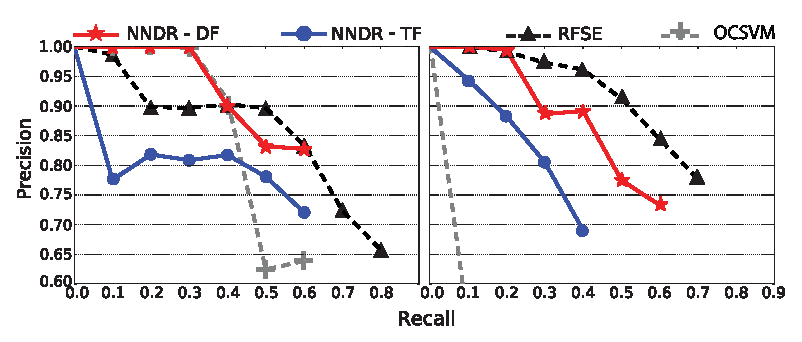
\includegraphics[scale=0.95]{NNDR_W3G-W1G_Best_RFSE-OCSVM-Baselines.eps}
	\caption{Precision curves in 11-standard recall levels of the examined open-set classifiers using either W3G features (left) or W1G features (right).}
	\label{fig:NNDR_W3G_Best_RFSE_Baseline}
	\end{center}
\vspace{-7mm}
\end{figure}

%, i.e. the remaining part after the last mark of each curve it the percentage of the corpus tha has been classified as Unknown from the algorithms.





\section{Experiments}\label{chap:word_embeddings:sec:experimental_setup}

\subsection{Open-set Evaluation Methodology}
In this study we are measuring the performance of a novel extension of the NN method, designed for open-set classification when the web-documents used as input are \textit{Distributional Encoding of Fixed Size Vectors} derived from an PVBOW NNet model. In particular we are measuring the effect the marked-as-unknown (or marked-as-noise) genre class tags, to the open-set prediction process.

To compensate the potentially unbalanced distribution of web pages over the genres, we are using the macro-averaged precision and recall measures. Than is a modified version of precision and recall for open-set classification tasks proposed by \parencite{mendesjunior2016}. This modification calculates precision and recall only for the known classes (available in the training phase) while the unknown samples (belonging to classes not available during training) affect false positives and false negatives. To find parameter settings that obtain optimal evaluation performances we use two scalar measures, the \textit{Area Under the Precision-Recall Curve} (AUC)and $F_{1}$. We will show that the appropriate selection of the optimization measure is highly significant in the presence of noise.

Precision-Recall curve is a standard method to visualize the performance of classifiers. In this paper, the Precision-Recall curve is calculated in 11-standard recall levels $[0,0.1,...,1.0]$. Precision values are interpolated based on the following formula:

\begin{equation}
	P(r_j)=max_{r_j \leqslant r \leqslant r_{j+1}}(P(r))
\end{equation}

\noindent
where $P(r_j)$ is the precision at $r_j$ standard recall level.

\subsection{Corpora}\label{chap:word_embeddings:sec:corpora}
In this paper we study NNRD performance with distributional features derived from a NNet PVBOW corpus. In particular, the open-set algorithms described above are analytically tested on benchmark corpus already used in previous work in WGI \parencitep{meyer2004genre,santini2007automatic,kanaris2009learning,pritsos2018open}, the \textit{SANTINIS} \parencite{mehler2010genres_on_web} corpus.Details are given in table \ref{tbl:genre_tags}. This is a corpus comprising 1,400 English web pages evenly distributed into 7 genres as well as 80 BBC web pages evenly categorized into 4 additional genres. In addition, it comprises a random selection of 1,000 English web pages taken from the SPIRIT corpus \parencite{joho2004spirit}. The latter can be viewed as noise in this corpus. In particular in this study SPIRIT tags are considered \textit{Marked as Unknown} (MU) and this is how we measure them.

Note that in the evaluation process we both measuring two kind classification-as-unknown of the open-set algorithm; the \textit{false positive unknown} where are classification of samples which have class tags known to the NNRD model and the \textit{true positive unknown} where they are marked-as-unknown (or marked-as-noise) where they are considered as noise.

\subsection{Settings}\label{chap:word_embeddings:sec:evaluation_measures}
Our text representation features are based exclusively on textual information from web pages excluding any structural information, URLs, etc. Based on the good results reported in \parencitep{sharoff2010web,pritsos2013open,Asheghi2015} as well as some preliminary experiments. The following document representation schemes are examined: Character 4-grams (C4G), Word unigrams (W1G), and Word 3-grams (W3G).

We use the Term-Frequency (TF) weighting scheme and Distributional Learning scheme. The feature space for TF is defined by a \textit{Vocabulary} which is extracted based on the terms appearing at training set only. The TF-Vocabulary range of dimensions have been tested are $V_{TF}\textit{=\{5k,10k,50k,100k\}}$. The feature space in the Distributional model is pre-selected while the deep learning process of PVBOW model. The range of the models fixed dimensions has been tested are $D_{dim}\textit{=\{50,100,250,500,1000\}}$ based of previews studies related to the distributional features on Natural Language Processing domain where relatively small dimensions are used, compare to TF scheme.

The DM vocabulary creation process is also driven by an internal terms \textit{vocabulary} which is used for eliminating the terms with lower than a preferred frequency and then discards the terms from the text window for the PVBOW (see section \ref{sec:Gensim}). In this study we have tested as the $TF_{min}=\{3,10\}$ minimum frequencies set. The text window tested was $P_{win}=\{3,8,20\}$ size set. In respect of PVBOW model, other (hyper-)parameter values put to a test were $\alpha=0.025$, $epochs=\{1, 3, 10\}$ and $decay=\{0.002, 0.02\}$.

Particularly for NNRD then following parameters have been tested:1) $\lamba\textit{=\{0.2, 0.5, 0.7\}}$ which is regulating the balance between the known and the unknown classification accuracy risk in the formula \ref{eq:NA}, 2)DRT threshold selection candidates $DRT\textit{=\{0.4, 0.6, 0.8, 0.9\}}$. Also two other parameters we have introduced in our implementation; the percentage of the training set to be split internally as Training/Validation sub-sets where $V_{ptg}\textit{=\{0.5, 0.7\}}$ has been tested. Then the percentage of the validation set which was split as unknown $U_{ptg}\textit{=\{0.3, 0.5\}}$ has been tested.

The Random Feature Sub-spacing Ensemble (RFSE) algorithm is a variation of the method presented by Koppel et al. \parencitep{koppel2011authorship} for the task of \textit{author identification}. In the original approach, there is only one training example for each author and a number of simple classifiers is learned based on random feature subspacing. Each classifier uses the cosine distance to estimate the most likely author. The key idea is that it is more likely for the true author to be selected by the majority of the classifiers since the used subset of features will still be able to reveal that high similarity.  That is, the style of the author is captured by many different features so a subset of them will also contain enough stylistic information. Since WGI is also a style-based text categorization task, this idea should also work for it.

In our study we adopt the RFSE method as introduced in \parencitep{pritsos2013open} shown in \textit{Algorithm \ref{alg:RFS-Ensemble}}. There are multiple training examples (documents) for each available genre. To maintain simplicity of classifiers, we have used a \textit{centroid vector} for each genre. In the training phase, a centroid vector is formed, for every class, by averaging all the Term-Frequency (TF) vectors  of the training examples of web pages for each genre.

The class centroids are all formed for a given feature type. Then, an evaluation document is compared against every centroid and this process is repeated $I$ times. Every time a different feature sub-set is used. Then, the scores are ranked from highest to lowest and we measure the number of times the document is top-matched with every class. The document is assigned to the genre with maximum number of matches given that this score exceed a predefined $\sigma$ threshold. In the opposite case, the document remains unclassified, the RFSE responds "I Don't Know".

As comparative \textit{Baseline} we have employed RFSE. With respect to RFSE, four parameters should be set: the vocabulary size $V_{F}$, the number of features used in each iteration $FSS$, the number of iterations \textit{I}, and the threshold $\sigma$. We examined, $FSS$=\textit{\{1k, 5k, 10k, 50k, 90k\}}, \textit{I}=\textit{\{10, 50, 100, 200, 300, 500, 1000\}} and $\sigma$\textit{=\{0.5, 0.7, 0.9\}}. Additionally, in this work we are testing three document similarity measures: cosine similarity. All these parameters have been selected as suggested in \parencite{pritsos2018open}.

Finally, to extract the best possible parameter settings for each classification method we apply grid-search over the space of all parameter value combinations.

\begin{table}
\center
\begin{tabular}{|l|l|}
\hline
\multicolumn{1}{|c|}{Genre} & \multicolumn{1}{c|}{Pages} \\
\hline
\multicolumn{1}{|l|}{Blog} & \multicolumn{1}{c|}{200}  \\
\multicolumn{1}{|l|}{Eshop} & \multicolumn{1}{c|}{200} \\
\multicolumn{1}{|l|}{FAQ} & \multicolumn{1}{c|}{200} \\
\multicolumn{1}{|l|}{Frontpage} & \multicolumn{1}{c|}{200} \\
\multicolumn{1}{|l|}{Listing} & \multicolumn{1}{c|}{200} \\
\multicolumn{1}{|l|}{Personal Home Page} & \multicolumn{1}{c|}{200} \\
\multicolumn{1}{|l|}{Search Page} & \multicolumn{1}{c|}{200} \\
\multicolumn{1}{|l|}{DIY Mini Guide (BBC)} & \multicolumn{1}{c|}{20} \\
\multicolumn{1}{|l|}{Editorial (BBC)} & \multicolumn{1}{c|}{20} \\
\multicolumn{1}{|l|}{Features (BBC)} & \multicolumn{1}{c|}{20} \\
\multicolumn{1}{|l|}{Short Bio (BBC)} & \multicolumn{1}{c|}{20} \\
\multicolumn{1}{|l|}{Noise (Spirit1000)} & \multicolumn{1}{c|}{1000}  \\
\hline
\end{tabular}
\caption {SANTINIS corpora descriptions and amount of pages per genre.}
\label{tbl:genre_tags}
\end{table}


\section{Results}\label{chap:word_embeddings:sec:Experiments_Results}

In this study we are evaluating the performance of NNDR algorithm into the open-set framework with the presence of noise, as the notion of noise explained above. That is we are only using the 11 known genre classes of SANTINIS corpus for training, while for evaluation we are using all 12 classes. The true genre class tags for the documents of the in the 12th class is not known and it is only considered as noise. Therefore, we have to deal with \textit{unstructured noise}. Additionally, since the noise-class is marked then the algorithm is evaluated in both false-positive classifications of the marked-unknown-classes as known an the false-negative classifications of the known-classes as unknown. In both cases the false classifications are causing a penalty to the Macro-F1 and Macro-Precision-Recall Curves we are using for evaluation.

We perform  10-fold cross validation and in each fold we include the full set of 1,000 pages of noise. This evaluation strategy is giving a more realistic evaluation. Since the noise size is greater than the size of any genre included in the given genres collection.

Initially we are comparing the performance of NNDR with RFSE on TF features vocabulary. RFSE returns higher score to NNDR, in tables \ref{tbl:NNDR_TF} and \ref{tbl:RFSE_TF}, for Macro-F1 and Macro-AUC and for any terms-type. Note also that the TF feature model dimensions for both algorithm is in all cases a few thousands.

\pagebreak

\begin{table}
\center
\begin{tabular}{|l|cccc|lr|rrrr|}
\hline
MAX. & STP & SUP & DRT & $\lambda$ & T.TYPE & DIMs & M\emph{P} & M\emph{R} & M\emph{AUC} & M\emph{F1} \\
\hline
F1 & 0.7 & 0.3 & 0.8 & any & C4G & 5000 & 0.664 & 0.403 & 0.291D & 0.502 \\
AUC & 0.7 & 0.3 & 0.8 & any & C4G & 5000 & 0.664 & 0.403 & 0.291D & 0.502 \\
F1 & 0.7 & 0.5 & 0.8 & any & W1G & 5000 & 0.691 & 0.439 & 0.348D & 0.537 \\
AUC & 0.7 & 0.5 & 0.8 & any & W1G & 5000 & 0.691 & 0.439 & 0.348D & 0.537 \\
F1 & 0.5 & 0.5 & 0.8 & 0.3 or 1.5 & W3G & 10000 & 0.720 & 0.664 & 0.486D & 0.691 \\
AUC & 0.5 & 0.5 & 0.6 & 0.5 & W3G & 5000 & 0.738 & 0.604 & 0.437D & 0.664 \\
\hline
\end{tabular}
\caption {Maximum performance of NNDR on TF Features of SANTINIS coprus. STP is the Spliting Training Percentage. SUP is the Splitting Unknown Percentage. DRT is the Distance Ration Threshold. $\lambda$ is the weigthing balance regulation parameters for the Normalized Accuracy. T.TYPE is the Terms Type. DIMs is the features model's dimensions. MP is the Macro Precision. MR is the Macro Recall. MAUC is the Area Under the Macro PR Curve. MF1 is the F1 score of the Macro Precision and Macro Recall.}
\label{tbl:NNDR_TF}
\end{table}

\begin{table}
\center
\begin{tabular}{|l|ccc|lr|rrrr|}
\hline
MAX. & FSS & $\sigma$T & ITER. & T.TYPE & DIMs & M\emph{P} & M\emph{R} & M\emph{AUC} & M\emph{F1} \\
\hline
F1 & 1000 & 0.5 & 100 & C4G & 50000 & 0.739 & 0.780 & 0.652 & 0.759 \\
AUC & 500 & 0.5 & 300 & C4G & 10000 & 0.686 & 0.831 & 0.722 & 0.751 \\
F1 & 10000 & 0.5 & 1000 & W1G & 50000 & 0.776 & 0.758 & 0.657 & 0.767 \\
AUC & 1000 & 0.5 & 300 & W1G & 5000 & 0.618 & 0.807 & 0.673 & 0.700 \\
F1 & 1000 & 0.7 & 100 & W3G & 50000 & 0.797 & 0.722 & 0.488 & 0.758 \\
AUC & 10000 & 0.5 & 100 & W3G & 100000 & 0.657 & 0.805 & 0.696 & 0.723 \\
\hline
\end{tabular}
\caption {Maximum performance of RFSE on TF Features of SANTINIS coprus. FSS is the Features Subset Selection number. $\sigma$T is the sigma threshold of the RFSE. ITER is the number of iterations of the RFSE. T.TYPE is the Terms Type. DIMs is the features model's dimensions. MP is the Macro Precision. MR is the Macro Recall. MAUC is the Area Under the Macro Precision-Recall Curve. MF1 is the F1 score of the Macro Precision and Macro Recall.}
\label{tbl:RFSE_TF}
\end{table}

\begin{table}
\center
\begin{tabular}{|l|cccc|lr|ccccr|rrrr|}
\hline
MAX. & STP & SUP & DRT & $\lambda$ & T.TYPE & DIMs & MTF & WS & $\alpha$ & EP. & DEC. & M\emph{P} & M\emph{R} & M\emph{AUC} & M\emph{F1} \\
\hline
F1 & any & any & 0.8 & any & C4G & 50 & 3 & 8 & 0.025 & 10 & 0.002 & 0.829 & 0.600 & 0.455D & 0.696 \\
AUC & any & any & 0.8 & any & C4G & 500 & 3 & 3 & 0.025 & 10 & 0.02 & 0.755 & 0.602 & 0.539D & 0.670 \\
F1 & any & any & 0.8 & any & W1G & 50 & 3 & 3 & 0.025 & 10 & 0.02 & 0.733 & 0.670 & 0.541D & 0.700 \\
AUC & any & any & 0.8 & any & W1G & 50 & 3 & 3 & 0.025 & 10 & 0.02 & 0.733 & 0.670 & 0.541D & 0.700 \\
F1 & any & any & 0.8 & any & W3G & 100 & 3 & 3 & 0.025 & 10 & 0.02 & 0.827 & 0.615 & 0.564D & 0.706 \\
AUC & any & any & 0.8 & any & W3G & 100 & 3 & 3 & 0.025 & 10 & 0.02 & 0.827 & 0.615 & 0.564D & 0.706 \\
\hline
\end{tabular}
\caption {Maximum performance of NNDR on Distributional Features of SANTINIS corpus. STP, SUP, DRT, $\lambda$, T.TYPE, DIMs are the same as in table \ref{tbl:NNDR_TF}. MTF is the Minimum Threshold Fequency of the Distributional models Vocabulary. WS is the Windows Size of the text sentence. $\alpha$ is the NNet parameter. EP is the epochs number of the NNet model. DEC is the decay parameter of the NNet model. MP is the Macro Precision. MR is the Macro Recall. MAUC is the Area Under the Macro PR Curve. MF1 is the F1 score of the Macro Precision and Macro Recall.}
\label{tbl:NNDR_Gensim}
\end{table}




However, there is a notable difference in the behavior of the two algorithms where it seems to be the reason RFSE outperforms NNDR. NNDR is using the 5000 (with the exception of line 4 of table \ref{tbl:RFSE_TF}) most frequent features for both training and evaluation phases. RFSE is using about 1000 \textit{randomly selected features} from the 50,000 to 100,000 most frequent features. This observations leading as the conclusion that the textual-genre information is pervasive in several features of the texts irrespectively of their frequency.

In order to research our null hypothesis where the textual-genre information is pervasive in the correlation of the features and not only in their frequency, we employee the distributional features explained above. Comparing tables \ref{tbl:NNDR_TF} and \ref{tbl:NNDR_Gensim} there is a notable improvement. Particularly for the Macro-F1 Score the performance reaches $0.7$ in all cases. Moreover, the STP, SUP and $\lambda$ parameters can my any of the set we have tested, on the contrary to the TF features model where only a specific value pare case is returning the maximum performance. Concerning TF model only when W3G terms-type is used we have a comparable $F1$ and $AUC$ value to the respective performance of the distributional model for NNDR.

We have also examined the case where $AUC$ is maximized because it seems in \parencite{pritsos2018open} study this measure is maximized when precision is maximized while the recall is kept as max as possible. As an example note line 6 at table \ref{tbl:NNDR_TF} where for W3G the precision can reach $0.738$ while recall only reduced to $0.604$ compare to the $0.664$ in the above line where F1 is maximized.

The open-set classification framework evaluation design naturally turns our interest to the precision performance of the algorithms. To reason it we have to consider that a classifier in a binary case should distinguish the \textit{known and the unknown web documents} are not belonging to the target class. In addition it has to recognize the the documents of the target class. Thus 2 out of 3 evaluation score naturally related to the precision score.

In precision perspective it seems NNDR with distributional features outperforms RFSE in all case. In addition the size of features models dimension are 10 to 200 times smaller. NNDR returns $0.829$ macro-precision score compare to $0.739$ of the RFSE, for C4G terms-type. Moreover, the maximum precision of RFSE is $0.797$ with $0.722$ recall while the respective recall for them maximum NNDR precision performance is $0.600$.

The performance of NNDR (with distributional features) increases for $10\%$ on average for precision and decreases for $21.00\%$ compare to the RFSE. In addition, its performance increases for $7\%$ in precision and $37\%$ in recall compare to it self when TF feature model is used.

We further evaluated the performance of NNDR in respect of precision performance and for this reason we have selected the best performance with the AUC criterion for NNDR using DF model, which in for this corpus is also maximizes $F1$. In figure \ref{fig:NNDR_W3G_Best_RFSE_Baseline} NNDR with DF, NNDR with TF and RFSE with TF are shown. All curves are showing the performance when W3G is used where it the case NNDR with DF is returning the maximum performance on SANTINIS corpus.

\begin{figure}[H]
\begin{center}
    \includegraphics[scale=0.99]{NNDR_W3G_Best_RFSE-Baseline_2.eps}
	\caption{Precision-Recall Curves of NNDR on SANTINIS corpus with RFSE as Baseline. The curves are for W3G terms-type and for AUC optimization criterion. The 11-recall-levels are shown for each evaluation experiment. The lines are stopping before the 11th recall level due to the open-set framework, i.e. the remaining part after the last mark of each curve it the percentage of the corpus tha has been classified as Unknown from the algorithms.}
	\label{fig:NNDR_W3G_Best_RFSE_Baseline}
	\end{center}
\end{figure}

The NNDR-DF is starting higher from all the curves and it remains to $0.99$ precision for the $30\%$ of the corpus then it drops to the same level with the RFSE baseline and after $0.50\%$ drops below it. However, it remains over $0.80$ up to $60\%$ of the corpus. The the rest of the corpus is classified as unknown. RFSE manages to recognize correctly part of the corpus up to $80\%$ with the precision to drop to $0.70$ and then to $0.65$. Considering the NNDR-TF is significantly lower in performance compare to the base line and is also has a significant drop in performance for the first $10\%$ of the corpus. Given that the curves are calculated based on the ranked scores from the best performance to the lowest performance it seems that the algorithm significantly affected by the noise of the marked-unknown part. That is the algorithm makes very confident decision for some part of the corpus confusing them with other classes. Its overall performance is over $0.7$ precision and still recognize the $60\%$ of the corpus.

To conclude it seems that distributional features are giving a significant increment in performance even for a pure performance and very algorithm as NN, particularly the NNDR, i.e. an open-set version of it. Still RFSE where has successfully used for  WGI and other NLP problems, is giving higher over all performance in respect of macro-F1 and AUC. However, in respect of precision which is naturally more important for an open-set evaluation set the distributional features are offering higher or equal performance with 100 times smaller feature size. Moreover, considering the open-set framework as a filtering-setup for the algorithms one would probably prefer the NNDR-DF algorithm over RFSE.

\section{Conclusions}\label{sec:conclusions}

In this paper we presented an experimental study where is focused on the effect of distributional features on an open-set web-page document classification task. In contrast to vast majority of previous work in this area, we adopt the open-set scenario that is more realistic for  web-page classification since it is not feasible to construct a genre palette with all available genres and appropriate samples for each one of them. Particularly we are evaluating the possible performance improvement of an open-set algorithm when distributional features are employed, using the SANTINIS corpus.

The open-set algorithm we have evaluated with distributional features input is a novel variation of Nearest Neighbors algorithm named NNDR. A Distance Ration threshold is calculated while the training procedure for maximizing the \textit{Normilized Accuracy} of the known and the unknown classes.

Our evaluation methodology previews shown to be proper for evaluation open-set scenarios. The natural focus in an open-set evaluation framework is the macro-precision, since always there is a part of the corpus will be classified as unknown. Either because it is unknown (marked-as-unknown) or it is considered as outage while training.

In our evaluation distributional feature are giving a great improvement to the NNDR algorithm compare to it TF features performance. Moreover comparing it to the RFSE algorithm, our baseline, there is also an improvement in respect of macro-precision with some cost to the recall performance. Overall NNDR from a very low performance compare to the baseline it is becoming a comparable choice.

As concerns the terms-types, either fo the TF features model of the distributional one in all cases W3G provided the maximum scores.
distributional
In this study we concluded that probably the distributional features is a prospective choice for the WGI research community. Thus, a farther research would be fruitful focusing on several important aspects the selection of the similarity measures other than cosine we have used. There are also several variation and parameters for the distributional features one can use, for instance we have used Bag-of-words-paragraph vectors for training on our NNet deep learning model.

Finally it almost became tradition to be underlined that there is a need for a well formed corpus specialized for the WGI task. We need larger corpora including multiple genre labels. In addition there is a need for a constant updating of this corpus to capture the new trends in the genre pallet of the web itself, since new genre classes are added and the current ones are rapidly changing context, as naturally the human communication is reformed in a temporal manner.


\section{Final VERSION}

\section{Proposed Approach --- Open-Set Web Genre Identification}~\label{sec:approach}


\subsection{Nearest Neighbors Distance Ratio Classifier}\label{sec:NNRD_Description}

The Nearest Neighbors Distance Ratio (NNRD) classifier is an open-set classification algorithm introduced in \parencite{mendesjunior2016}, which in turn, is an extension upon the \textit{Nearest Neighbors} (NN) algorithm. NNRD calculates the distance of a new sample $s$ to its nearest neighbor $t$ and to the closest training sample $u$ belonging to a different class with respect to $t$. Then, if the ratio $d(s,t)/d(s,u)$ is higher than a threshold, the new sample is classified to the class of $s$. Otherwise, it is left unclassified. 

It is remarkable that, in contrast to other open-set classifiers, training of NNDR requires both known samples (belonging to classes known during training) and unknown examples (belonging to other/unknown classes) of interest. In more details, the \textit{Distance Ratio Threshold} (DRT) used to classify new samples is adjusted by maximizing the \textit{Normalized Accuracy} (NA)  $NA = \lambda A_{KS} + (1 - \lambda) A_{US}$, where $A_{KS}$ is the accuracy on known samples and $A_{US}$ is the accuracy on unknown samples. The parameter $\lambda$ regulates the mistakes trade-off on the known and unknown samples prediction. Since usually in training phase only known classes are available, Mendes et al. \parencite{mendesjunior2016} propose an approach to repeatedly split available training classes into two sets (known and "simulated" unknown). In our implementation of NNDR, we use cosine distance rather than the Euclidean distance because previous work found this type of distance more suitable for WGI \parencite{pritsos2018open}.\footnote{\url{https://github.com/dpritsos/OpenNNDR}}

